\documentclass{standalone}
\usepackage{tikz}
\usetikzlibrary{shapes, arrows, positioning, calc}

\begin{document}
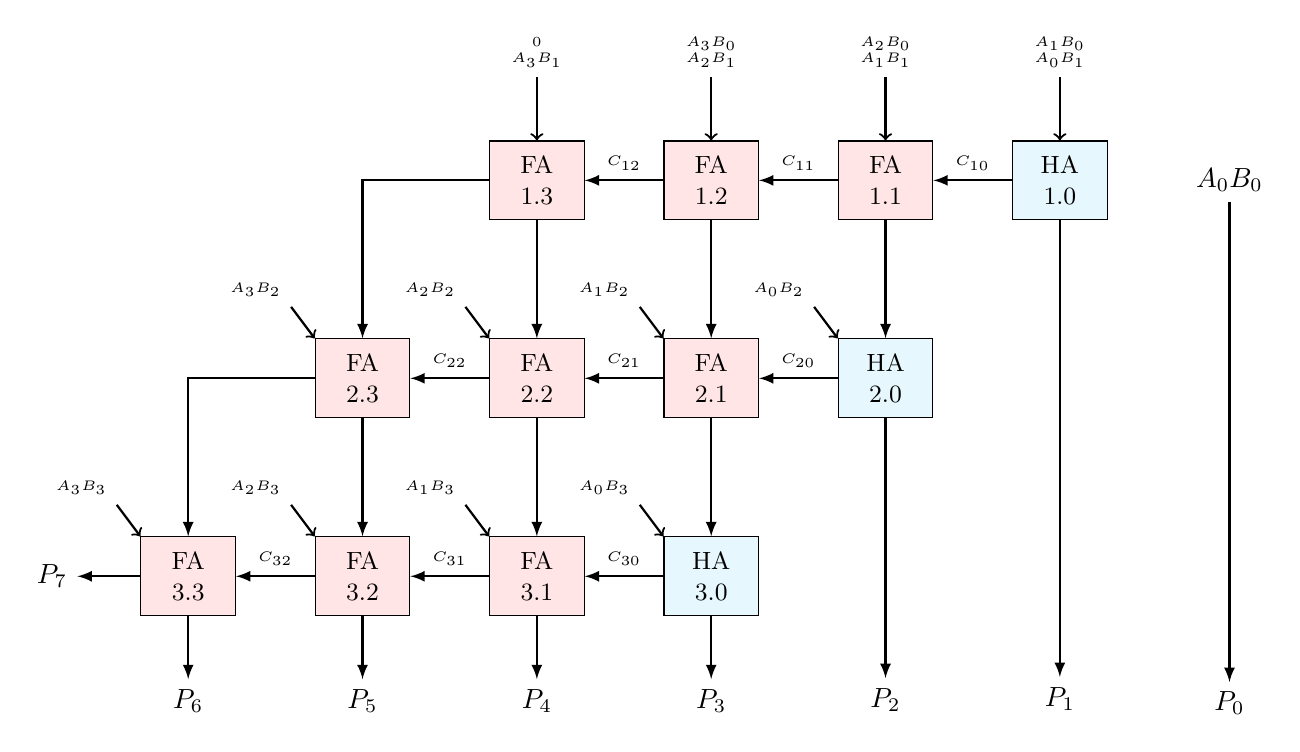
\begin{tikzpicture}[
    node distance=1.5cm and 1.0cm,
    auto,
    % Styles
    block/.style={draw, rectangle, align=center, minimum width=1.2cm, minimum height=1cm, inner sep=0pt, font=\small},
    ha/.style={block, fill=cyan!10},
    fa/.style={block, fill=red!10},
    wire/.style={->, >=latex, thick},
    label_text/.style={font=\tiny, align=center}
]

    % --- ROW 1 ---
    % LSB is on the Right.
    % HA10 (Bit 1, Col 1)
    \node[ha] (HA10) at (0, 0) {HA\\1.0};
    
    % FA11 (Bit 2, Col 2) - Left of HA10
    \node[fa, left=of HA10] (FA11) {FA\\1.1};
    
    % FA12 (Bit 3, Col 3) - Left of FA11
    \node[fa, left=of FA11] (FA12) {FA\\1.2};
    
    % FA13 (Bit 4, Col 4) - Left of FA12
    \node[fa, left=of FA12] (FA13) {FA\\1.3};


    % --- ROW 2 ---
    % HA20 (Bit 2, Col 2) - Below FA11
    \node[ha, below=of FA11] (HA20) {HA\\2.0};
    
    % FA21 (Bit 3, Col 3) - Below FA12
    \node[fa, below=of FA12] (FA21) {FA\\2.1};
    
    % FA22 (Bit 4, Col 4) - Below FA13
    \node[fa, below=of FA13] (FA22) {FA\\2.2};
    
    % FA23 (Bit 5, Col 5) - Left of FA22
    % This takes C13. C13 comes from FA13. So it makes sense to be left of FA22 (visually next msb).
    \node[fa, left=of FA22] (FA23) {FA\\2.3};


    % --- ROW 3 ---
    % HA30 (Bit 3, Col 3) - Below FA21
    \node[ha, below=of FA21] (HA30) {HA\\3.0};
    
    % FA31 (Bit 4, Col 4) - Below FA22
    \node[fa, below=of FA22] (FA31) {FA\\3.1};
    
    % FA32 (Bit 5, Col 5) - Below FA23
    \node[fa, below=of FA23] (FA32) {FA\\3.2};
    
    % FA33 (Bit 6, Col 6) - Left of FA32
    \node[fa, left=of FA32] (FA33) {FA\\3.3};


    % --- EXTERNAL INPUTS (P0) ---
    % P0 corresponds to A0B0. It bypasses everything.
    % Let's place a node right of HA10.
    \node[right=of HA10] (P0_in) {$A_0 B_0$};
    \node[below=6.1cm of P0_in] (P0_out) {$P_0$};
    \draw[wire] (P0_in) -- (P0_out);


    % --- ROW 1 CONNECTIONS ---
    
    % Carries (Right to Left)
    \draw[wire] (HA10) -- node[above, font=\tiny] {$C_{10}$} (FA11);
    \draw[wire] (FA11) -- node[above, font=\tiny] {$C_{11}$} (FA12);
    \draw[wire] (FA12) -- node[above, font=\tiny] {$C_{12}$} (FA13);
    
    % Inputs (Top)
    \draw[<-, thick] (HA10.north) -- ++(0,0.8) node[above, label_text] {$A_1 B_0$\\$A_0 B_1$};
    \draw[<-, thick] (FA11.north) -- ++(0,0.8) node[above, label_text] {$A_2 B_0$\\$A_1 B_1$};
    \draw[<-, thick] (FA12.north) -- ++(0,0.8) node[above, label_text] {$A_3 B_0$\\$A_2 B_1$};
    \draw[<-, thick] (FA13.north) -- ++(0,0.8) node[above, label_text] {$0$\\$A_3 B_1$};

    % Outputs (Down)
    % HA10 Sum -> P1
    \draw[wire] (HA10.south) -- ++(0, -5.8) node[below] {$P_1$};
    
    % FA11 Sum -> HA20 Input
    \draw[wire] (FA11.south) -- (HA20.north);
    % FA12 Sum -> FA21 Input
    \draw[wire] (FA12.south) -- (FA21.north);
    % FA13 Sum -> FA22 Input
    \draw[wire] (FA13.south) -- (FA22.north);
    
    % FA13 Cout -> FA23 Input. This is tricky.
    % Visually FA23 is to the left of FA22 in Row 2.
    % FA13 is above FA22.
    % FA13 Cout connects to FA23 "A" input (top).
    % Let's route it diagonally or explicitly.
    \draw[wire] (FA13.west) -- ++(-1.5, 0) -| (FA23.north);


    % --- ROW 2 CONNECTIONS ---
    
    % Carries
    \draw[wire] (HA20) -- node[above, font=\tiny] {$C_{20}$} (FA21);
    \draw[wire] (FA21) -- node[above, font=\tiny] {$C_{21}$} (FA22);
    \draw[wire] (FA22) -- node[above, font=\tiny] {$C_{22}$} (FA23);
    % FA23 Cout is C23, goes to FA33.
    
    % Inputs (Side/Top) for additional partial products
    % HA20 takes A0 B2
    \draw[<-, thick] (HA20.north west) -- ++(-0.3, 0.4) node[above left, label_text] {$A_0 B_2$};
    % FA21 takes A1 B2
    \draw[<-, thick] (FA21.north west) -- ++(-0.3, 0.4) node[above left, label_text] {$A_1 B_2$};
    % FA22 takes A2 B2
    \draw[<-, thick] (FA22.north west) -- ++(-0.3, 0.4) node[above left, label_text] {$A_2 B_2$};
    % FA23 takes A3 B2
    \draw[<-, thick] (FA23.north west) -- ++(-0.3, 0.4) node[above left, label_text] {$A_3 B_2$};

    % Outputs (Down)
    % HA20 Sum -> P2
    \draw[wire] (HA20.south) -- ++(0, -3.3) node[below] {$P_2$};
    
    % FA21 Sum -> HA30
    \draw[wire] (FA21.south) -- (HA30.north);
    % FA22 Sum -> FA31
    \draw[wire] (FA22.south) -- (FA31.north);
    % FA23 Sum -> FA32
    \draw[wire] (FA23.south) -- (FA32.north);
    
    % FA23 Cout -> FA33 Input
    \draw[wire] (FA23.west) -- ++(-0.5, 0) -| (FA33.north);


    % --- ROW 3 CONNECTIONS ---
    
    % Carries
    \draw[wire] (HA30) -- node[above, font=\tiny] {$C_{30}$} (FA31);
    \draw[wire] (FA31) -- node[above, font=\tiny] {$C_{31}$} (FA32);
    \draw[wire] (FA32) -- node[above, font=\tiny] {$C_{32}$} (FA33);
    
    % Inputs (Side/Top)
    % HA30 takes A0 B3
    \draw[<-, thick] (HA30.north west) -- ++(-0.3, 0.4) node[above left, label_text] {$A_0 B_3$};
    % FA31 takes A1 B3
    \draw[<-, thick] (FA31.north west) -- ++(-0.3, 0.4) node[above left, label_text] {$A_1 B_3$};
    % FA32 takes A2 B3
    \draw[<-, thick] (FA32.north west) -- ++(-0.3, 0.4) node[above left, label_text] {$A_2 B_3$};
    % FA33 takes A3 B3
    \draw[<-, thick] (FA33.north west) -- ++(-0.3, 0.4) node[above left, label_text] {$A_3 B_3$};

    % Outputs (Down) - Valid Product Bits
    \draw[wire] (HA30.south) -- ++(0, -0.8) node[below] {$P_3$};
    \draw[wire] (FA31.south) -- ++(0, -0.8) node[below] {$P_4$};
    \draw[wire] (FA32.south) -- ++(0, -0.8) node[below] {$P_5$};
    \draw[wire] (FA33.south) -- ++(0, -0.8) node[below] {$P_6$};
    \draw[wire] (FA33.west) -- ++(-0.8, 0) node[left] {$P_7$};

\end{tikzpicture}
\end{document}
